\section{Introduction}

% UMTS Network

% RRC State Machine
3G cellular data networks have recently witnessed rapid growth, especially due to the emergence of smartphones. In this paper, we focus on the\textit{ Universal Mobile Telecommunications System} (UMTS) 3G network, which is among the most popular 3G mobile communication technologies. However, the bottleneck of the internet resides in the first hop of the network, and large amount of lower layer retransmission could cause significant latency~\cite{bufferbloat}. 3G network has a bad reputation at the initial period of network connection~\cite{3g.slow}, and significant delay will hurt user experience badly. In this paper, we are going to allocate the fundamental cause of the abnormal latency, and propose a modified protocol solution.

3G network systems operate under radio resource constraints. To efficiently utilize the limited radio resources, UMTS introduces for each \textit{user equipment} (UE, i.e. smartphone) a \textit{radio resource control} (RRC) state machine, such as in Figure~\ref{fig:rrc.state.machine}, that determines radio resource usage affecting device energy consumption and user experience~\cite{spec-3G-RRC}. UE will stay in one of three states, each with different amount of allocated radio resources. The transitions between states also have significant impact on the UMTS system.

\begin{figure}
\centering
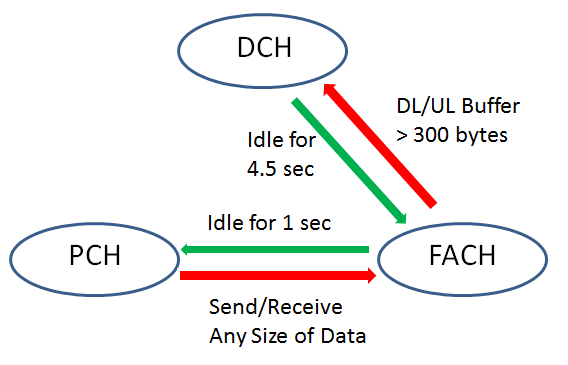
\includegraphics[width=0.45\textwidth]{figs/rrc_state.png}
\caption{RRC State Machine for the 3G UMTS network for T-Mobile}
\label{fig:rrc.state.machine}
\end{figure}

The network topology provides a nature isolation between different layers. The design of transport layer protocol doesn't require the knowledge of lower layer information. However, the abstraction of the design could lead to sub-optimal scenario, i.e. large significant latency will occur during the RRC state transition. Since the root cause of the abnormal delay behavior resides in the data link layer (i.e. RLC, radio link control, layer), the visibility of lower layer information will help us identify the root cause of the bizarre behavior in upper layer. 

Previous studies~\cite{3g_rrc, 4g_rrc, aro, opt.tcp.rlc} don't have accessibility to detailed link layer data transmission information, so they have to treat the lower layer as a black box, and use inference technique to determine and control RRC states with less accuracy. In our study, the QxDM tool is able to capture the fine grained data transmission and context information (i.e. signal strength, RLC protocol configuration) in both upper and lower layers. To the best of our knowledge, our study is the first cross-layer analysis that have both ground truth knowledge in transport layer and data link layer. Thanks to our cross-layer visibility, we identify the root cause of the unexpected latency as the RLC protocol's lagging response to the packet loss signal. We propose \emph{Fast Re-Tx} as the improved RLC layer mechanism to reduce the latency over the initial data transmission. We summarize our contributes here:

\begin{itemize}
\item \textbf{Novel cross-layer mapping mechanism to fully correlate multiple network layers.} We develop the first cross-layer mapping algorithm that accurately maps the TCP/UDP packets to the corresponding \textit{packet data unit} (PDU) in the RLC layer. Our mapping accuracy is on average 99.8\%.
\item \textbf{Root cause analysis on the performance issue and propose feasible solutions.} Based on the cross-layer mechanism, we could perform an in-depth analysis on RLC layer behavior during the initial data transmission period. We found that the RLC sender doesn't reactive to PDUs loss signal --- duplicate \textit{acknowledgement} (ACK) PDUs, and it leads to upper layer packet delays, and even TCP \textit{retransmission timeout} (RTO). Therefore, we propose RLC \emph{Fast Re-Tx} to actively respond to duplicate RLC ACK PDUs to reduce the latency over problematic initial data transmission period. We evaluate the improved mechanism using real time traces, and estimate the RLC \textit{round-trip time} (RTT) could drop up to 35.69\% over FACH state.
\end{itemize}

%Therefore, cross-layer analysis over QxDM logs would help us have a in-depth understanding the correlation between different layers, and identify the root cause of abnormal latency behaviors during the initial state of data transmission.

%\begin{figure}
%\centering
%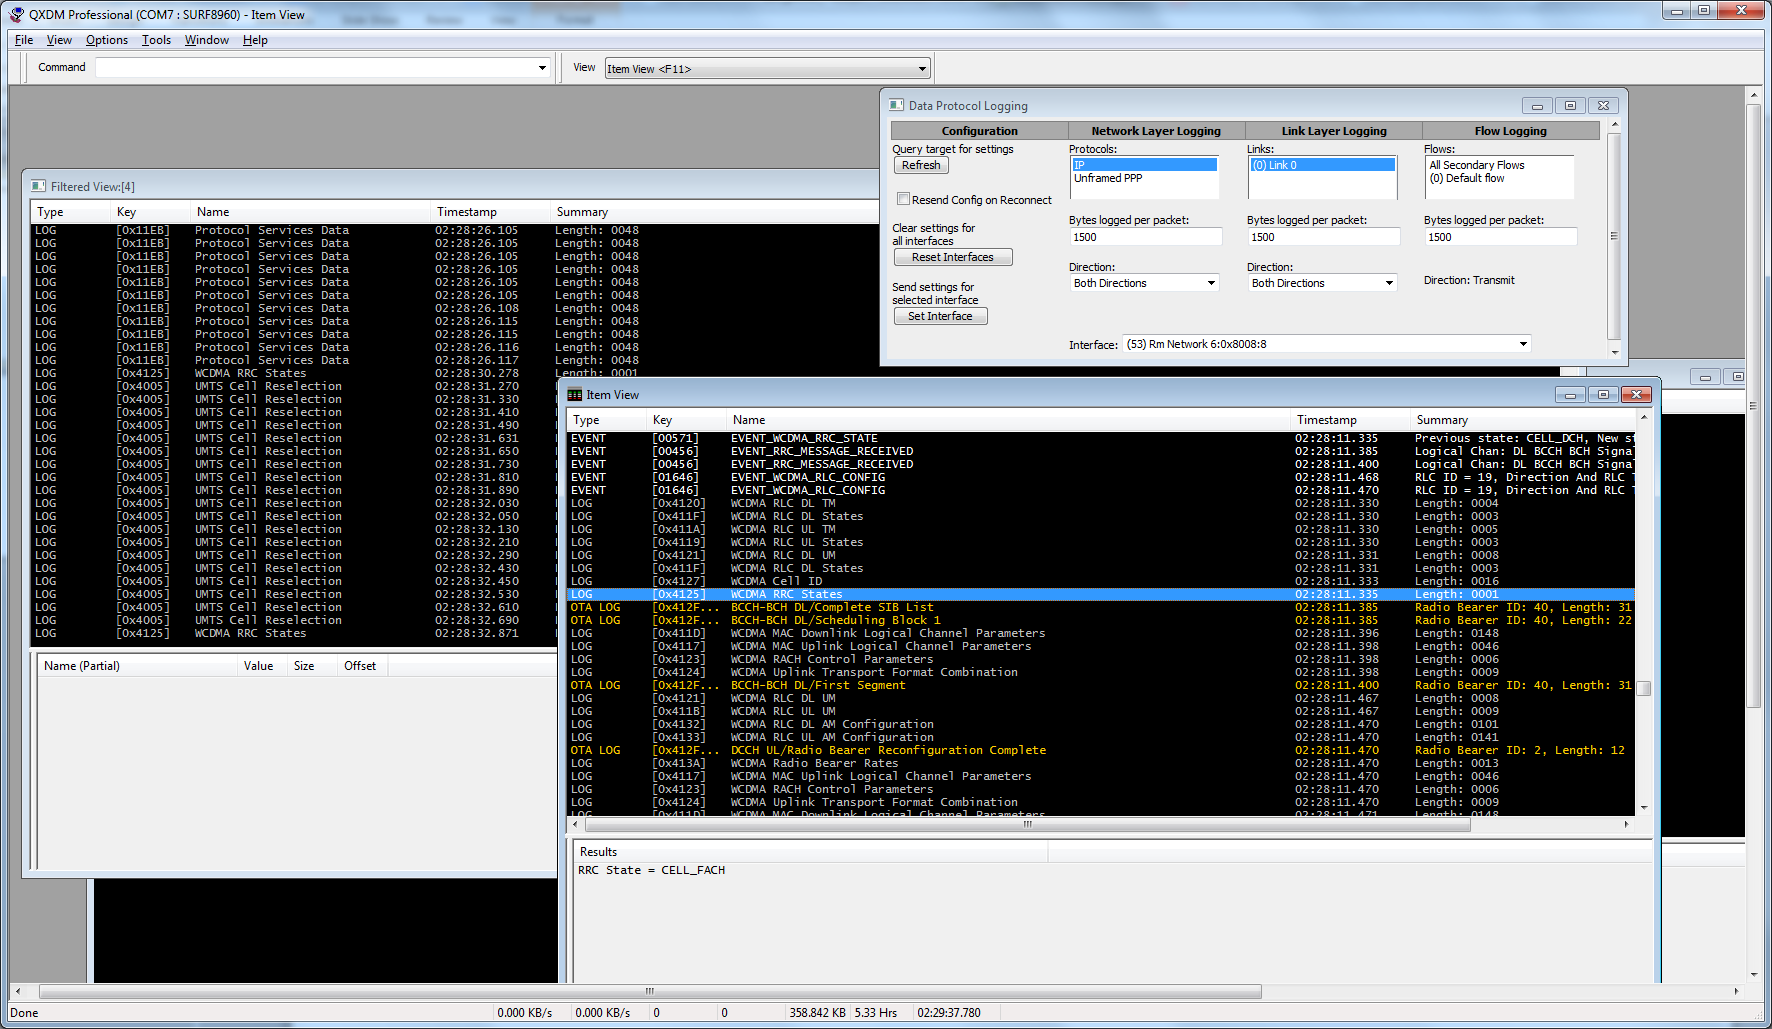
\includegraphics[width=0.45\textwidth]{figs/QxDM.png}
%\caption{Ongoing monitoring and logging activities on QxDM}
%\label{fig:qxdm}
%\end{figure}

\label{sec:intro}

